To complement and validate the results of the offline evaluation,  we ran a user study with 24 subjects to measure the performance of users with different clustering algorithms for an interactive visual interface.  In the following, we first describe the user study methodology followed by an evaluation of user performance.

\subsection{Methodology}
The main goal of this user study was to ask students to find the natural disasters in our collection of tweets. Before starting the experiment, each user was introduced to the goal of the survey with a video describing the interface and the different features. Then, each user was trained using two different search algorithms to find three different natural disasters using both a baseline interface showing all results as well as a clustering interface.

In brief, the user study interface allows users to enter a search query with results shown on an interactive Google Maps display used to browse the results. 
The tweets that match a query were represented using circles with a grayscale color range corresponding to the probability of relevance -- light gray circles represented low probability relevance tweets, and dark gray circles represented high probability relevance tweets.
The user was able to interact with the map by panning, zooming and dragging and also by clicking on tweets and clusters to view their content (for clusters, we display a summary in terms of selected keywords).
The user could also use a time slider bar to restrict the results to tweets matching the query in a specific time window. 
Once each user had familiarized themselves with the interface, they were asked to find three other natural disasters using a different display algorithm (baseline, K-means, EF1 relevance-driven clustering using the BPS greedy algorithm) for each of three trials containing three natural disasters each. 

In each trial, the user was asked to enter information related to each natural disaster they identified, including the type of the natural disaster, its location (US state), and the date on which they think the disaster happened. We collected detailed interaction logs to record different behaviors and actions of the user. Moreover, each user was asked to answer NASA Task Load Index (NASA-TLX)~\cite{HART1988139} and System Usability Scale (SUS)~\cite{brooke1996sus} questionnaires after each trial. Finally, at the end of the experiment, each user was asked to fill out an exit survey, which included a ranking of the algorithms.

The three algorithms used to drive the interface in this user survey were:
\begin{enumerate}
\item A baseline method which displays all tweets that match the query (an example is shown in  Figure~\ref{Fig:GlobalDisplay}).
\item The BPS algorithm we proposed for relevance-driven clustering which displays the top 6 clusters for a query (an example is shown in Figure~\ref{Fig:FilteredDisplay}).
\item The K-Means algorithm discussed previously in the offline evaluation (using X-Means to automatically identify the best $K$), which also displays the top 6 clusters for a query (an example is shown in Figure~\ref{fig:ScreenShot}).
\end{enumerate}

Note that the probability relevance score of each tweet was derived using a language model to estimate $S(j)$~\cite{Zhai2001}.
Also, for each user the sequence of algorithms to evaluate was presented differently, such that to cover all possible six combinations uniformly four times (24 users).  Here, we wish to indicate that the user had no indication of what algorithm was used each time, especially between the BPS and the K-Means algorithms, which both present the results in a similar way using clusters (bounding boxes). 
%Finally, we highlight the fact that during we have set up the task such that it wasn't too easy nor too difficult for the user. 
A total of 24 users participated in our user study, for which the experiment took on average 50 minutes per user.

Figure \ref{fig:ScreenShot} shows the interface of the user study, with the results of the query ``tornado, blizzard, earthquake''  using K-Means. The results of the same query with the baseline and the BPS algorithms are shown in Figure \ref{Fig:UseCase}. At first glance, we clearly observe that the clusters of the BPS algorithm are more focused and more contextualized than those of the K-Means algorithm.  In the following, we analyze the main outcomes of this user study.



\begin{figure}[t]
\begin{centering}
{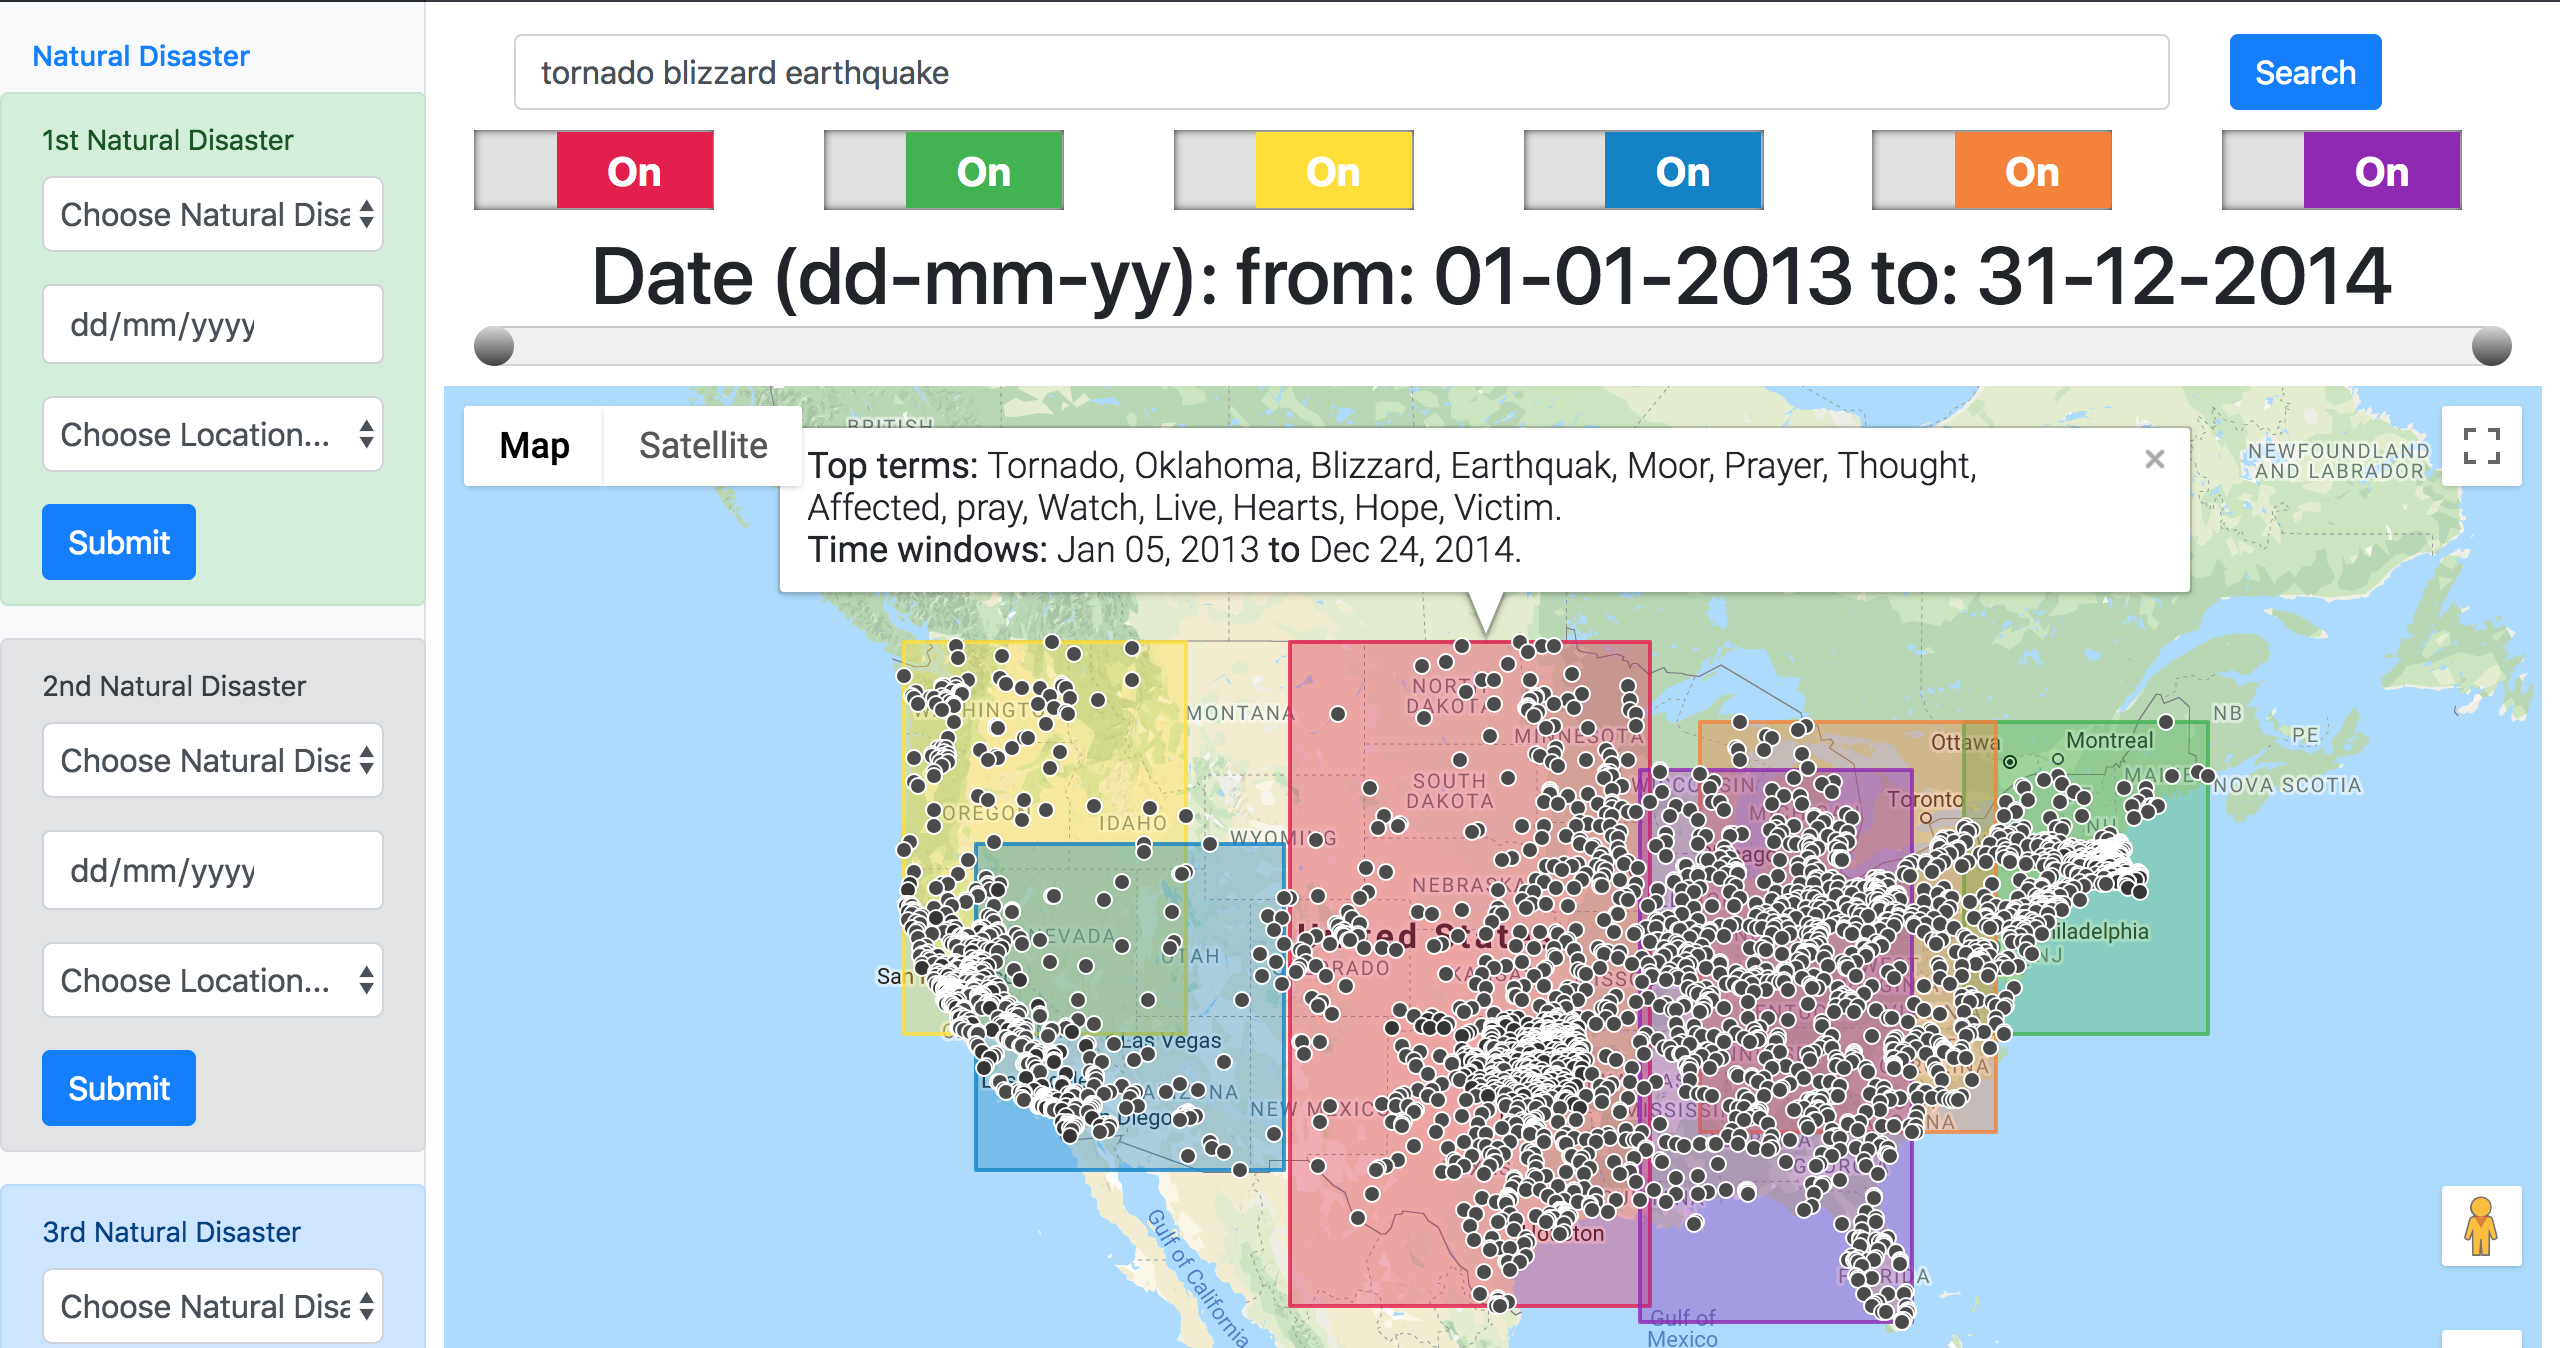
\includegraphics[width=8.5cm]{imgs/kmeans}}
\par\end{centering}
\caption{User survey Web page. The results of the query ``tornado, blizzard, earthquake''  are shown using clusters of X-Means, which can be hidden/shown using the buttons at the top. The sidebar was used to provide answers.}
\label{fig:ScreenShot}
\end{figure}


\begin{figure}[t]
\begin{centering}

\includegraphics[width=7.5cm]{imgs/legend3}
\par\end{centering}
\begin{centering}
{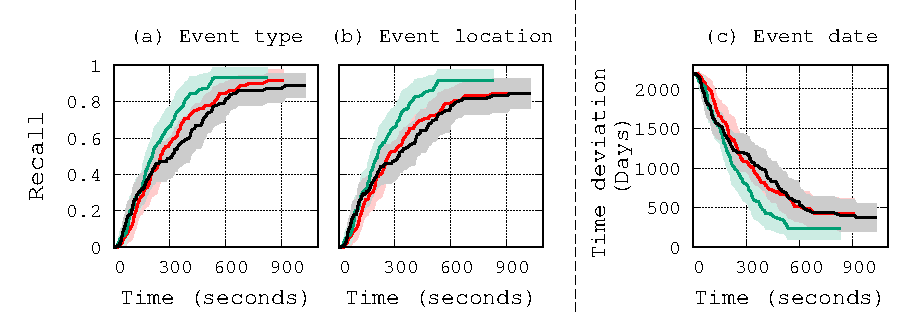
\includegraphics[width=8.5cm]{imgs/nd_recall}}
\par\end{centering}
\caption{The mean user performance and 95\% confidence intervals for each of the three search interfaces/algorithms are measured using cumulative recall for the type and location of the natural disasters and the absolute error for the first date of the natural disaster.  On average, users achieved higher recall and lower error faster using relevance-driven clustering (BPS) in comparison to K-means and the Baseline system.}
\label{fig:UserSurveyRecall}
\end{figure}





%However, 
\begin{figure*}[t]
\begin{centering}

\includegraphics[width=7.5cm]{imgs/legend4}\\
\subfigure[Natural disasters.] {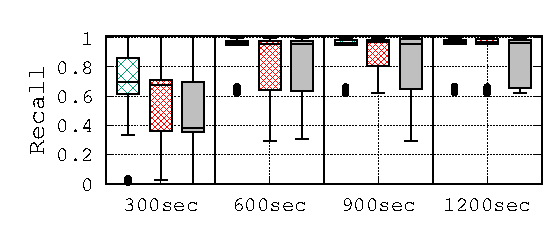
\includegraphics[width=5.7cm]{imgs/nd_recall_steps}}
\subfigure[Locations of the natural disasters.] {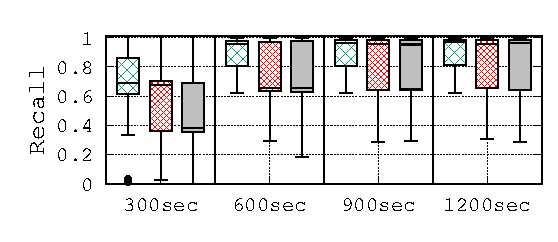
\includegraphics[width=5.7cm]{imgs/location_recall_steps}}
\subfigure[Errors in the dates of the natural disasters.] {\includegraphics[width=5.7cm]{imgs/nd_time_deviation_recall_steps}}
\par\end{centering}
\caption{Performance of the algorithms measured at different elapsed times for each trial.}
\label{fig:UserSurveyRecallStage}
\end{figure*}



\subsection{Performance analysis}

The performance of the users for each algorithm was measured using cumulative recall for the type and location of the natural disasters in each trial.  We remark that there were three distinct natural disasters per trial so perfect recall would require getting all three natural disaster types or locations correct.  Mean performance across all users for cumulative recall of disaster type and location are respectively shown in Figures~\ref{fig:UserSurveyRecall}(a) and Figure~\ref{fig:UserSurveyRecall}(b).  Users also had to enter their estimated starting date of each natural disaster, which we measure by absolute error assuming the maximum amount of error for any natural disasters that have not been submitted yet.  The mean performance of time estimation error across all users is reported in Figure~~\ref{fig:UserSurveyRecall}(c).  Moreover, in Figure~\ref{fig:UserSurveyRecallStage} we report the progression of these metrics for each algorithm using boxplots at different elapsed times into the experiment -- at 300, 600, 900 and 1200 seconds.

In brief, the main outcome of this performance analysis are fairly straightforward: 
%(i) 
From Figure~~\ref{fig:UserSurveyRecall}, we see that on average, users achieved higher task recall and lower error faster when using the BPS algorithm for relevance-driven clustering in comparison to K-Means and the baseline.
% The performance obtained for this user study confirms clearly the results obtained in the off-line evaluation since the BPS algorithm outperforms K-Means and the baseline in identifying the natural disasters, their locations, and their dates.
%(ii) In general, the clustering approach is clearly useful for this kind of task as both BPS and K-Means outperformed the baseline that show all matching elements. 
%(iii) Clearly, the BPS algorithm required much fewer efforts and time to complete the task than for K-Means and the baseline and that to reach a bit higher level of recall.
%(iv) 
Further considering the performance progression shown in Figure~\ref{fig:UserSurveyRecallStage}, we clearly notice that with the BPS algorithm, participants were able to achieve a higher performance at early stage of the experiment than using the two other algorithms. 

% As a conclusion for this evaluation, we notice that there is a similar outcome between the two evaluation methods -- the offline evaluation and the user study. Both evaluations confirm that the BPS algorithm
% the significant contribution of the BPS algorithm for this specific relevance-driven clustering task. Even though the off-line evaluation showed that K-Means is inappropriate for this task, the performance obtained in this user study showed that it is effective to some extent. 

\begin{figure}[t]
\begin{centering}

\includegraphics[width=7.5cm]{imgs/legend4}\\
\subfigure[Subscales rating. %``0'' means the user thinks that the workload for the considered dimension was ``Low'' and ``20'' means it was ``High''.
] {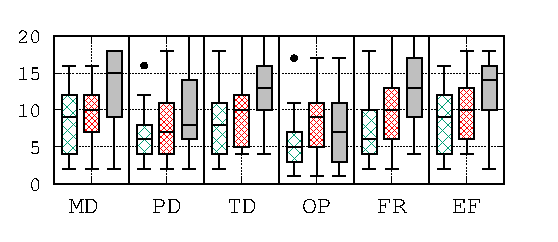
\includegraphics[width=4.6cm]{imgs/NASA_TLX}}
\subfigure[Overall rating.] {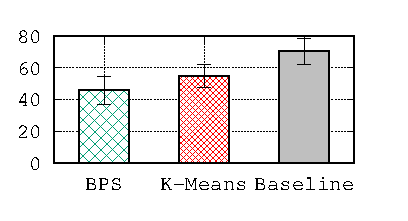
\includegraphics[width=3.8cm]{imgs/NASA_TLX_AVERAGE}}
\par\end{centering}
\caption{NASA Task Load Index (MD: Mental Demand, PD: Physical Demand, TD: Temporal Demand, OP: Own Performance, FR: Frustration, EF: Effort). }
\label{fig:NASA}
\end{figure}



\subsection{Surveys analysis}

With the previously discussed quantitative measures of user performance indicating the advantage of relevance-driven clustering, we next proceed to evaluate the users' own opinions of each interface/algorithm as collected in the user surveys discussed in the methodology.

During this user study, each participant had to answer 7 different questionnaires -- a NASA Task Load Index (NASA-TLX)~\cite{HART1988139} and a System Usability Scale (SUS)~\cite{brooke1996sus} questionnaires after having used each algorithm, plus a final questionnaire. We report below the main outcomes of each survey.




\subsubsection{NASA-TLX analysis}

The NASA-TLX questionnaire rates perceived workload in order to assess a task, system effectiveness or other aspects of performance.
The questionnaire includes questions on mental demand, physical demand, temporal demand, performance, frustration, and effort. NASA-TLX items are rated on a 20-point scale (1 = low workload, 20 = high workload, except for OP where 1 = perfect and 20 = failure). 
We show the NASA-TLX results obtained  for each subscale and for the overall ratings  in Figure~\ref{fig:NASA}.
Briefly, the mean overall NASA-TLX rating was $45.91\pm 8.86$ for BPS, $54.75\pm 7.41$ for K-Means, and $70.41\pm 8.27$ for the baseline. 
A Friedman's test revealed an overall significant difference ($\chi^2(3)= 16.113, p=0.003 < 0.05$).
Holm-Bonferroni corrected post-hoc analyses with Wilcoxon signed-rank tests 
revealed that the difference between all pairs was significant ($p < 0.05$). %The difference between BPS and K-Means wasn't significant. Moreover, there were no significant differences in the sub-scales between BPS and K-Means.


According to these results, we note that participants overall perceived the BPS algorithm to be more effective at helping them complete their search task in comparison to using K-Means or the baseline.  Global median rates of frustration and mental effort were around 10, which indicates that the task was neither too difficult, nor too easy.  Also, as the median rates of these two factors were lower for the two clustering methods than the baseline, we conclude that participants overall felt that clustering-based search provided a less frustrating and less mentally demanding interface for this task in comparison to the baseline, which displayed all search results. 
Finally, based on the task load rates where the BPS algorithm performed the best, we believe that relevance-driven clustering provided the most effective approach for carrying out this kind of geo-temporal search task.

\begin{figure}[t]
\begin{centering}

\includegraphics[width=7.5cm]{imgs/legend4}
{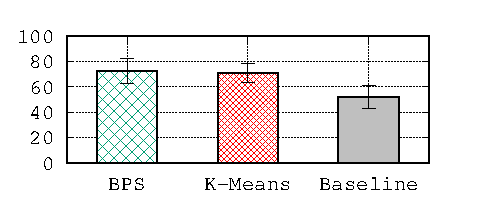
\includegraphics[width=7.5cm]{imgs/SUS_AVERAGE}}
\par\end{centering}
\caption{System Usability Scale overall rating.}
\label{fig:SUS}
\end{figure}

\subsubsection{SUS analysis}
The SUS questionnaire gives a global view of subjective assessments of usability. The questionnaire contains questions related to the global effectiveness, efficiency, and satisfaction. The SUS items are rated on a 5-point scale (0 = strong disagreement and 5 = strong agreement). In Figure~\ref{fig:SUS}, we show the results obtained over all SUS scores  with 95\% confidence interval . The mean SUS score was $72.39\pm 9.77$ for BPS, $70.83\pm 7.61$ for K-Means, and $51.77\pm 9.07$ for the baseline. A Friedman's test revealed an overall significant difference ($\chi^2(3)= 9.053, p=0.010 < 0.05$).
Holm-Bonferroni corrected post hoc analyses with Wilcoxon signed-rank tests 
revealed that the difference between the two clustering methods and the baseline  was significant ($p < 0.05$). The difference between BPS and K-Means wasn't significant and hence we can only infer from the SUS survey that the users preferred the clustering interface (i.e., BPS and K-Means) over the baseline display of all search results.


\subsubsection{Final questionnaire analysis}
The final questionnaire that the participants had to answer included questions on the advantages and disadvantages of each algorithm, plus a global ranking of the three algorithms. %Due to space limitations, we briefly summarize the top disadvantages of the BPS algorithm and advantages of the baseline method in Table~\ref{tbl:SurveyComments}.




% Preview source code for paragraph 0

%\begin{table}
%\caption{User survey comments.}
%\label{tbl:SurveyComments}
%\begin{centering}
%\begin{tabular}{|>{\centering}p{4cm}|>{\centering}p{4cm}|}
%\hline 
%\textbf{Disadvantages of BPS} & \textbf{Advantages of Baseline}\tabularnewline
%\hline 
%\hline 
%Clusters that have huge time-spend are most likely useless. & Simple, easy. Using %just the time sliders it was very easy to detect
%the disasters. \tabularnewline
%\hline 
%Does not show up all the data points.  & Using the timeslider, I found it more %useful than the filters. \tabularnewline
%\cline{1-1} 
%The interface takes more time to learn.  & \tabularnewline
%\hline 
%\end{tabular}
%\par\end{centering}
%\end{table}






The ranking of the algorithms provided by participants is shown in Figure \ref{fig:UserSurveyRanking}. 
We note that 18 participants out of 24 ranked  BPS as being the best algorithm, and 19 participants out of 24 ranked the baseline approach as being the least helpful for this task.  Hence there is strong evidence for user preference of BPS over K-means and for both BPS and K-means over the baseline system.  
%However, we note that two users mentioned that they still prefer the baseline approach. 
%This is probably due to the fact that they are used to work with a conventional search approach, and that they couldn't digest this new search clustering paradigm. 
Finally, we mention that in the surveys, several participants reported the utility, the ease and the precision provided by the BPS algorithm to complete this search task.














\begin{figure}[t]
\begin{centering}

\includegraphics[width=7.5cm]{imgs/legend4}\\
{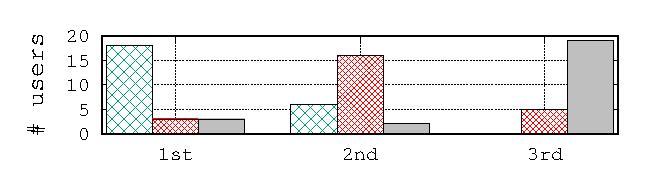
\includegraphics[width=8cm]{imgs/ranking}}
\par\end{centering}
\caption{Ranking of the algorithms by participants.}
\label{fig:UserSurveyRanking}
\end{figure}







